
Pharmaceutical supply chain (PSC) concerns the process of sourcing raw materials, manufacturing, distributing, and delivering medications to patients~\cite{SHAH2004929}. It is a complex process that includes various stakeholders and requires careful coordination and adherence to regulatory guidelines at every stage to ensure patients receive safe and effective medications.
%
PSC is especially critical in the case of oncological treatments due to the consequences of shortages on treatment quality~\cite{Nonzee2018,McBride2022}, and challenging due to the high degree of therapy personalization~\cite{ZUGAZAGOITIA20161551} that calls for
the on-demand preparation of drugs and accurate timing in the
distribution and delivery process. 
%
Moreover, patients can receive the treatment only after blood assessments. This can delay the administration and require to dynamically adapt the whole process.
%
PSC management is then very difficult to optimize since it needs to be responsive to sudden change while at the same time efficient in terms of costs and usage of resources.

Generally speaking, the PSC process involves the capability of tracking in real-time different kinds of physical assets (patients, therapy, vehicles, etc.), in different locations and with their own dynamics, enacting a process according to a plan that may need to be promptly revised and adapted depending on events and situations that concern those assets.

In this context, \acp{DTE} can be envisioned as a uniform approach to model and manage the ecosystem of heterogeneous physical assets involved in the oncologic PSC, enabling the development of smart digital systems to help achieve the proper level of responsiveness and adaptability. 


%=======================================================
\section{Case Study and Challenges}
%=======================================================
The diffusion of cancers and the consequent expenditure burden of cancer care, requires an effective management of the whole PSC \cite{Chen2023}.
%
This work focuses on the downstream of the process, namely, it is not interested in the enterprise production pipeline, but mainly in the in-loco drug preparation and timely administration~\cite{Papalexi2020}. 

For this work, the case study of the Istituto Romagnolo per lo Studio dei Tumori ``Dino Amadori''(IRST) has been analyzed.  IRST is a research centre located in Emilia-Romagna, Italy involved in the assistance and care for oncologic and onco-haematologic patients. IRST manage the whole PSC for more than 5.000 patients each year and registers more than 49,000 accesses for treatments. Oncologic pharmaceutic laboratories prepare more than 61,700 therapies by using more than 430 active substances. 
%
In this context, the process of preparation for cancer treatment begins after the medical prescription and patient's condition assessment, it involves multiple sub-tasks related to purchasing, stocking, picking, manipulating, scheduling and delivering treatment to the patient (in Hospital or other administration settings). 
%
It is a very complex process that should be optimized to reduce waste and guarantee a secure, right, and timeliness drug administration.
%
The main challenges are the following:
\begin{itemize}
    \item \textit{Optimized warehouse management:} Maintaining stock levels that respect the physical constraints of available spaces and provide precise information on the value (including forecasts) of materials in the warehouse is essential for efficient resource management.
    
    \item \textit{Right-time logistics:} Organizing, adapting, and monitoring transport to both input and administration sites must ensure punctuality and precision, guaranteeing safety and quality of care access for patients.
    
    \item \textit{Traceability and accountability:} The entire process must ensure traceability of materials and procedures, as well as accountability for the professionals involved, to enable continuous process review and rapid, accurate reconstruction of any incidents.
    
    \item \textit{Anticipation of information:} Digitizing the process ensures information is available at all times, and connecting different phases enables the anticipation of accurate data for planning subsequent steps.
    
    \item \textit{Level of automation:} The use of robots for efficient and safe production requires seamless interfacing between automation tools and information systems to support the process.
    
    \item \textit{Scenario simulation:} Oncology treatments are frequently updated with new guidelines and administration configurations, and varying costs of active ingredients impact organizational sustainability. The ability to simulate the effects of new therapeutic opportunities is therefore crucial for professionals involved in planning.
    
    \item \textit{Clinical trials:} Prescribing, confirming, preparing, administering, and monitoring therapies in clinical trials requires special attention and high levels of safety and traceability to ensure successful research outcomes.
\end{itemize}


%=======================================================
\section{Workflow Analysis}
%=======================================================

A typical care center is organized as follows:
\begin{itemize}
    \item \textit{Production Units} are responsible for preparing treatments, generally assembling personalized packages by mixing active ingredients to produce individualized dosages, as well as including ancillary drugs and other medical equipment necessary for the treatment. The process is only partially automatable (using fully automated production lines), since manual operations and checks are required, especially for experimental treatments.

    \item \textit{Warehouses} store active ingredients, drugs, and other relevant medical equipment to be used in the production units. They may be physically separated from the production units and hierarchically organized to move required stocks from larger centralized warehouses to smaller local ones.

    \item \textit{Blood test facilities} collect samples from patients and analyze them to verify their suitability for the next iteration of therapy. Sampling and analysis may be carried out in different locations, requiring the transport of samples to the appropriate laboratory.

\end{itemize}

Patients undergoing therapy typically follow monthly treatment plans, which are prepared and administered after a blood test to help medical staff assess the effectiveness of the therapy and determine suitability for a new round of (either the same or a different) treatment.
%
In the reference context, patients are called into therapy delivery facilities, where blood samples are collected.
%
Samples are then analyzed in a separate laboratory. Production of the treatment begins as soon as results are positive, aiming to deliver the therapy as quickly as possible, so patients can wait at the care center and do not need to be given another appointment.

Given the strict time requirements for the overall process, it is clear that information should be tracked to ensure consistency and availability at all times, enabling an understanding of whether primary resources are available and whether the production process can handle upcoming requests.
%
Moreover, effective tracking of resources, ongoing therapies, and patient conditions could support better planning of appointments, selecting the ideal time for patients to come and be checked to both maximize the probability they can receive treatment and minimize trips to care centers, as well as optimize the overall utilization of center resources such as hospital beds.
%
Not only patients but also stockpile management in warehouses can be improved. This is critical because medical equipment and drugs often have expiration dates and special conservation requirements, such as temperature thresholds that must be maintained even during transport between facilities.

Finally, the scenario described is, of course, an ideal setting. Medical staff may need to adjust or entirely re-evaluate therapy based on patient reactions, impacting the overall process. Additionally, advancements in oncological research can introduce new experimental treatments that must be considered.
%
The system needs not only to track the current situation but also to react to unexpected variables and allow simulation of new scenarios.

%=======================================================
\section{\acl{DTE} Proposal}
%=======================================================

Having identified the complex nature of supply chain management for oncologic treatments, this work proposes a model for a \ac{DTE} to improve the tracking of resources in production and distribution processes.

Figure \ref{fig:model} illustrates the Digital Twins that compose the system and the main data each of them tracks to map the supply-chain process.
%
A minimum set of entities is selected to be reified as Digital Twins for system implementation. Patients, treatments, production units, and warehouses are modeled as Digital Twins.
%
Their roles and responsibilities are described in the following paragraphs.
%
Blood test and therapy delivery facilities are considered outside the scope of live tracking and are indirectly monitored through their interaction with the patient.
%
Future extensions of the system could include these facilities as well as the medical staff involved in treatment delivery for a more comprehensive overview.

\begin{figure}[t]
    \centering
    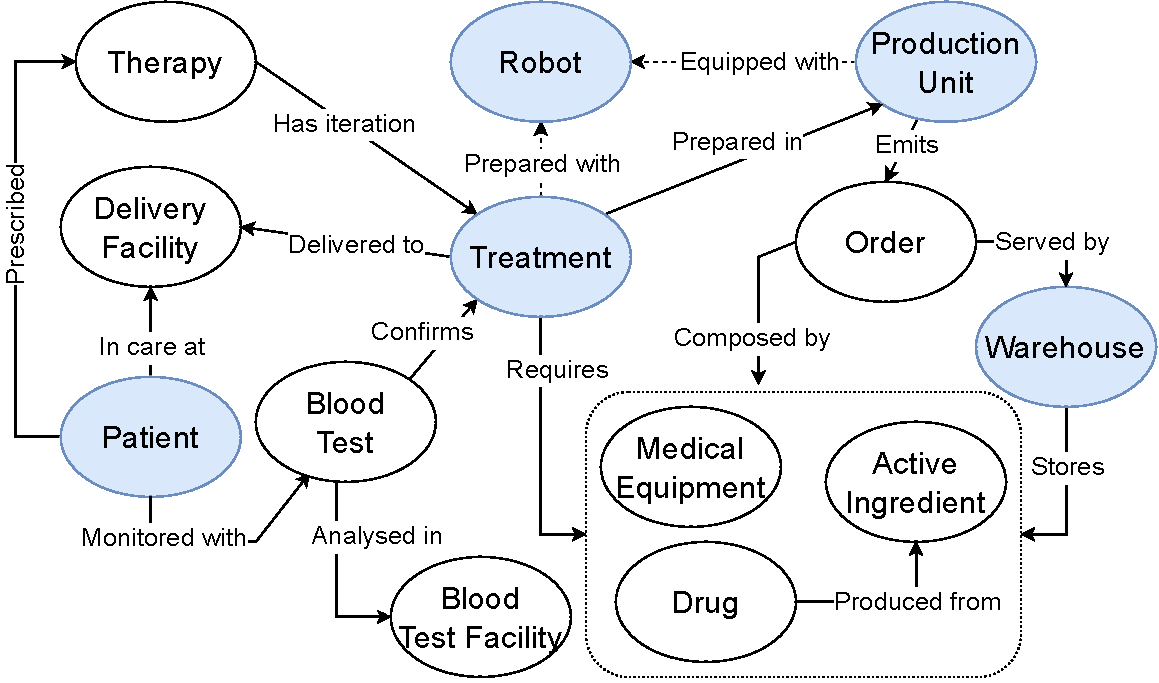
\includegraphics[width=0.9\textwidth]{figures/applications/CompressedDTModel.pdf}
    \caption{Entities in the system and their relationships, blue ellipsis represent the ones selected to be reified as Digital Twins.}
    \label{fig:model}
\end{figure}

\paragraph{Patient Digital Twin} tracks patient personal data, prescribed therapies, and periodic blood tests to monitor suitability for new treatments.
%
The Patient Digital Twin also records the delivery facility where the patient is receiving care, supporting resource utilization monitoring.
%
It can provide prediction services to forecast patient conditions, typically assessed with blood tests, and schedule subsequent treatment iterations accordingly. 
%
This service is detailed in the next section.

\paragraph{Treatment Digital Twin} exhibits the most dynamic behavior and is used to track the entire process, following its evolution and interactions with other system components.
%
Each Treatment Digital Twin begins in a \texttt{scheduled} state for a given date based on the therapy, then transitions to a \texttt{confirmed} state if the corresponding blood test is positive. 
%
This initiates the production process, with the treatment \texttt{assigned} to a production unit depending on local resource availability and current production capacity. 
%
Each Treatment Digital Twin stores information about required materials and is linked to the actual resources used in production to ensure batch tracking.
%
The Digital Twin then moves to a \texttt{production} state during preparation and, once ready, to a \texttt{distribution} state, tracking its transport to the therapy delivery facility where the patient is in care. 
%
Finally, it transitions to a \texttt{delivered} state once the treatment is administered.

\paragraph{Production Unit Digital Twin} monitors and estimates the production capability of a unit, allowing planning algorithms to distribute treatments and optimize selected performance indicators.
%
When treatments are assigned to a production unit, necessary resources must be retrieved from warehouses, prompting the production unit to issue shipment orders. 
%
This Digital Twin should provide simulation services to evaluate the impact of new requests or production failures on overall unit efficiency.

\paragraph{Warehouse Digital Twin} monitors stockpiles of medical equipment, active ingredients, and ready-to-deliver drugs, tracking stored quantities, expiration dates, and environmental conditions required for special resources.  
%
This Digital Twin can issue warnings if stocks fall below set thresholds, expiration dates approach, or required environmental conditions are not met, enabling new orders or resource redistribution to minimize waste. 

\medskip

Listing \ref{lst:kg-irst} presents the representation in Turtle syntax for RDF of the data collected by the system. 
%
The HL7 FHIR\footnote{\url{http://hl7.org/fhir}} standard is adopted as it provides a comprehensive vocabulary for electronic health records and facilitates interoperability of collected data.
%
Using FHIR resources, therapies for each patient are modeled as \texttt{CarePlan} resources and treatments as \texttt{MedicationRequest} resources, which can be fulfilled by a \texttt{SupplyRequest} handled during production and distribution, and a \texttt{MedicationAdministration} to represent where and how the produced treatment is administered during an \texttt{Encounter}.

\begin{code}
\captionof{listing}{Knowledge Graph representing a model of the data collected by the \ac{DT} system in FHIR RDF.}
\label{lst:kg-irst}
\inputminted{turtle}{listings/applications/KG_Partial.ttl}
\end{code}

The resulting \ac{KG} enables accurate recording of all events tracked during patient therapy. By using a standard vocabulary, the data is guaranteed to be interoperable and enriched with useful semantics.
%
This data can then be used to measure and monitor process KPIs, as well as to train models and make predictions.


Each \ac{DT} can host knowledge-based and data-driven models of the \ac{PA}.
These can be used to simulate scenarios, predict future states, and optimize processes.
%
To experimentally develop a Patient \ac{DT}, a data-driven model that includes anthropometric, cancer characteristics, blood-test results, treatment history, and recent lab values and was trained to predict the patient suitability for the next therapy cycle.

A dataset containing 12,045 patients was used to train the model using a 70/30 split. SVM, Random Forest, and AdaBoost models were trained for a binary task: predict whether the next blood test will be positive.
%
Despite model performance not being sufficient for conclusive results (probably due to dataset imbalance)
this prototype served the purpose of demonstrating the feasibility of embedding predictive models in \acp{DT} to enhance the overall system.
%
Refined models could be embedded in the Patient \ac{DT} to predict treatment readiness in advance, reducing wasted tests and staff time, minimizing patient wait and transport, improving warehouse and drug-preparation efficiency, and enabling more effective PSC planning.
